% Created 2022-11-07 Mon 21:57
% Intended LaTeX compiler: pdflatex
\documentclass[11pt]{article}
\usepackage[utf8]{inputenc}
\usepackage[T1]{fontenc}
\usepackage{graphicx}
\usepackage{longtable}
\usepackage{wrapfig}
\usepackage{rotating}
\usepackage[normalem]{ulem}
\usepackage{amsmath}
\usepackage{amssymb}
\usepackage{capt-of}
\usepackage{hyperref}
\graphicspath{{../../books/}}
% TIPS
% \substack{a\\b} for multiple lines text





% pdfplots will load xolor automatically without option
\usepackage[dvipsnames]{xcolor}

\usepackage{forest}
% two-line text in node by [two \\ lines]
% \begin{forest} qtree, [..] \end{forest}
\forestset{
  qtree/.style={
    baseline,
    for tree={
      parent anchor=south,
      child anchor=north,
      align=center,
      inner sep=1pt,
    }}}
%\usepackage{flexisym}
% load order of mathtools and mathabx, otherwise conflict overbrace

\usepackage{mathtools}
%\usepackage{fourier}
\usepackage{pgfplots}
\usepackage{amsthm, mathabx,  amsmath, commath}
\usepackage{amsfonts}

\usepackage{empheq}
\usepackage{tikz}
\usetikzlibrary{arrows.meta}
\usepackage[most]{tcolorbox}

\newtheorem{theorem}{Theorem}[section]
\newtheorem{definition}{Definition}[section]
\newtheorem{corollary}{Corollary}[section]
\newtheorem{example}{Example}[section]
\newtheorem{lemma}{Lemma}[section]
\newtheorem{proposition}{Proposition}[section]

\newcommand{\bl}[1] {\boldsymbol{#1}}
\newcommand{\Wt}[1] {\stackrel{\sim}{\smash{#1}\rule{0pt}{1.1ex}}}
\newcommand{\wt}[1] {\widetilde{#1}}


%For boxed texts in align, use Aboxed{}
%otherwise use boxed{}

\DeclareMathSymbol{\widehatsym}{\mathord}{largesymbols}{"62}
\newcommand\lowerwidehatsym{%
  \text{\smash{\raisebox{-1.3ex}{%
    $\widehatsym$}}}}
\newcommand\fixwidehat[1]{%
  \mathchoice
    {\accentset{\displaystyle\lowerwidehatsym}{#1}}
    {\accentset{\textstyle\lowerwidehatsym}{#1}}
    {\accentset{\scriptstyle\lowerwidehatsym}{#1}}
    {\accentset{\scriptscriptstyle\lowerwidehatsym}{#1}}
}

\usepackage{graphicx}
    
% text on arrow for xRightarrow
\makeatletter
%\newcommand{\xRightarrow}[2][]{\ext@arrow 0359\Rightarrowfill@{#1}{#2}}
\makeatother


\def \bx {\boldsymbol{x}}
\def \ba {\boldsymbol{a}}
\def \bI {\boldsymbol{I}}
\def \bt {\boldsymbol{t}}
\def \bb {\boldsymbol{b}}
\def \bA {\boldsymbol{A}}
\def \bX {\boldsymbol{X}}
\def \bu {\boldsymbol{u}}
\def \bS {\boldsymbol{S}}
\def \bZ {\boldsymbol{Z}}
\def \bz {\boldsymbol{z}}
\def \by {\boldsymbol{y}}
\def \bw {\boldsymbol{w}}
\def \bT {\boldsymbol{T}}
\def \bS {\boldsymbol{S}}
\def \bm {\boldsymbol{m}}
\def \bW {\boldsymbol{W}}
\def \bY {\boldsymbol{Y}}
\def \bH {\boldsymbol{H}}
\def \blambda {\boldsymbol{\lambda}}
\def \bPhi {\boldsymbol{\Phi}}
\def \btheta {\boldsymbol{\theta}}
\def \bmu {\boldsymbol{\mu}}
\def \bphi {\boldsymbol{\phi}}
\def \bSigma {\boldsymbol{\Sigma}}
\def \lb {\left\{}
\def \rb {\right\}}
\def \caln {\mathcal{N}}
\def \dissum {\displaystyle\Sigma}
\def \dispro {\displaystyle\prod}
\def \E {\mathbb{E}}
\def \Q {\mathbb{Q}}
\def \V {\mathbb{V}}
\def \R {\mathbb{R}}
\def \calq {\mathcal{Q}}
\def \calg {\mathcal{G}}
\def \caln {\mathcal{N}}
\def \calr {\mathcal{R}}
\def \calm {\mathcal{M}}
\def \calc {\mathcal{C}}
\def \bcup {\bigcup}

\makeindex
\usepackage[UTF8]{ctex}
\author{wu}
\date{\today}
\title{Trivial Big Data}
\hypersetup{
 pdfauthor={wu},
 pdftitle={Trivial Big Data},
 pdfkeywords={},
 pdfsubject={},
 pdfcreator={Emacs 28.0.92 (Org mode 9.6)}, 
 pdflang={English}}
\begin{document}

\maketitle
\tableofcontents


\section{一元线性回归}
\label{sec:org86d6c6d}
方差
\begin{equation*}
S^2_x=\frac{1}{n}\sum_{i=1}^n(x_i-\barx)^2
\end{equation*}
标准差
\begin{equation*}
S_x=\sqrt{\frac{1}{n}\sum_{i=1}^n(x_i-\barx)^2}
\end{equation*}
协方差
\begin{equation*}
Cov=\frac{1}{n}\sum_{i=1}^n(x_i-\barx)(y_i-\bary)
\end{equation*}
相关系数
\begin{equation*}
\rho=\frac{Cov}{S_xS_y}
\end{equation*}

一元线性回归:找一条直线,拟合数据点
\begin{equation*}
y=\beta_0+\beta_1x
\end{equation*}
最小二乘法
\begin{equation*}
\min_{\beta_0,\beta_1}\sum_{i=1}^n((\beta_0+\beta_1x_i)-y_i)^2
\end{equation*}

\begin{equation*}
f(\beta_0,\beta_1)=\sum_{i=1}^n((\beta_0+\beta_1x_i)-y_i)^2
\end{equation*}

\begin{align*}
&\frac{\partial f}{\partial\beta_0}=2\sum_{i=1}^n(\beta_0+\beta_1x_i-y_i)=0\\
&\Rightarrow n\beta_0+\beta_1\sum_{i=1}^nx_i-\sum_{i=1}^ny_i=0\\
&\Rightarrow\beta_0+\beta_1\barx-\bary=0
\end{align*}

\begin{gather*}
\frac{\partial f}{\partial\beta_1}=2\sum_{i=1}^nx_i(\beta_0+\beta_1x_i-y_i)=0\\
\sum_{i=1}^nx_i(\beta_0+\beta_1x_i-y_i)=0
\end{gather*}

注意到
\begin{equation*}
\sum_{i=1}^n\barx(\beta_0+\beta_1x_i-y_i)=\barx(n\beta_0+\beta_1\sum x_i-\sum y_i)=0
\end{equation*}
所以
\begin{equation*}
\sum_{i=1}^n(x_i-\barx)(\beta_0+\beta_1x_i-y_i)=0
\end{equation*}
而
\begin{equation*}
\sum_{i=1}^n(x_i-\barx)(\beta_0+\beta_1\barx-\bary)=(\beta_0+\beta_1\barx-\bary)\sum_{i=1}^n(x_i-\barx)=0
\end{equation*}
所以
\begin{equation*}
\sum_{i=1}^n(x_i-\barx)(\beta_1(x_i-\barx)-(y_i-\bary))=0
\end{equation*}
\begin{align*}
\beta_1&=\frac{\sum_{i=1}^n(x_i-\barx)(y_i-\bary)}{\sum_{i=1}^n(x_i-\barx)^2}=
\frac{\frac{1}{n}\sum_{i=1}^n(x_i-\barx)(y_i-\bary)}{\frac{1}{n}
\sum_{i=1}^n(x_i-\barx)^2}=\frac{Cov}{S_x^2}\\
&=
\frac{\frac{1}{n}\sum_{i=1}^n(x_i-\barx)(y_i-\bary)}
{\sqrt{\frac{1}{n}\sum_{i=1}^n(x_i-\barx)^2}\sqrt{\frac{1}{n}\sum_{i=1}^n(y_i-\bary)^2}}
\frac{\sqrt{\frac{1}{n}\sum_{i=1}^n(y_i-\bary)^2}}{\sqrt{\frac{1}{n}\sum_{i=1}^n(x_i-\barx)^2}}=
\rho\frac{S_y}{S_x}
\end{align*}
因此
\begin{equation*}
y=\bary-\beta_1\barx+\beta_1x\Rightarrow y-\bary=\beta_1(x-\barx)=\rho\frac{S_y}{S_x}(x-\barx)
\end{equation*}

\section{多元线性回归}
\label{sec:org1d83bbd}
\begin{equation*}
y=\beta_0+\beta_1x_1+\dots+\beta_mx_m
\end{equation*}
最小二乘法
\begin{equation*}
\min_{\beta_0,\dots,\beta_m}\sum_{i=1}^n((\beta_0+\beta_1x_{i1}+\dots+\beta_mx_{im})-y_i)^2
\end{equation*}
令
\begin{equation*}
\beta=
\begin{pmatrix}
\beta_0\\\beta_1\\\vdots\\\beta_m
\end{pmatrix}\hspace{1cm}
X=
\begin{pmatrix}
1&x_{11}&x_{12}&\dots&x_{1m}\\
1&x_{21}&x_{22}&\dots&x_{2m}\\
\vdots&\vdots&\vdots&\dots&\vdots\\
1&x_{n1}&x_{n2}&\dots&x_{nm}\\
\end{pmatrix}\hspace{1cm}
y=
\begin{pmatrix}
y_1\\y_2\\\vdots\\y_n
\end{pmatrix}
\end{equation*}
最小二乘形式
\begin{equation*}
\min_{\beta}\norm{X\beta-y}^2
\end{equation*}

\begin{equation*}
g(\beta)=\la w,\beta\ra=w^T\beta=\sum_{i=0}^mw_i\beta_i
\end{equation*}

\begin{equation*}
\nabla g=
\begin{pmatrix}
\frac{\partial g}{\partial \beta_0}\\
\frac{\partial g}{\partial \beta_1}\\
\vdots\\
\frac{\partial g}{\partial \beta_m}\\
\end{pmatrix}=
\begin{pmatrix}
w_0\\w_1\\\vdots\\w_m
\end{pmatrix}=w
\end{equation*}

假设\(A=A^T\)
\begin{equation*}
h(\beta)=\la A\beta,\beta\ra=\beta^TA\beta=\sum_{i,j}a_{ij}\beta_i\beta_j
\end{equation*}
定义\(p(u,v)=\la Au,v\ra=\la Av,u\ra\)
令
\begin{equation*}
u(\beta)=\beta,v(\beta)=\beta\Rightarrow h(\beta)=p(u(\beta),v(\beta))
\end{equation*}
\begin{equation*}
\nabla h=\frac{\partial p}{\partial u}\frac{\partial u}{\partial\beta}+\frac{\partial p}{\partial v}\frac{\partial v}{\partial \beta}=Av(\beta)+Au(\beta)=2A\beta
\end{equation*}

\begin{align*}
f(\beta)&=(X\beta-y)^T(X\beta-y)\\
&=(\beta^TX^T-y^T)(X\beta-y)\\
&=\beta^TX^TX\beta-\beta^TX^Ty-y^TX\beta+y^Ty
\end{align*}

\begin{equation*}
\nabla_\beta f=2X^TX\beta-X^Ty-X^Ty=2(X^TX\beta-X^Ty)=0
\end{equation*}

因此
\begin{equation*}
\beta=(X^TX)^{-1}X^Ty
\end{equation*}

为了增加鲁棒性,通常会最小化如下目标函数
\begin{equation*}
\norm{X\beta-y}^2+\lambda\norm{\beta}^2(\lambda>0)
\end{equation*}
此时
\begin{equation*}
\beta=(X^TX+\lambda I)^{-1}X^Ty
\end{equation*}

\section{逻辑回归}
\label{sec:orgf56edb9}
分类问题建模:
\begin{gather*}
f:\R^m\to\{0,1\}\\
f(x)=\sigma(\beta^Tx)
\end{gather*}
\(\sigma\)的一种取法:
\begin{equation*}
\sigma(z)=
\begin{cases}
1&z\ge 0\\
0&z<0
\end{cases}
\end{equation*}
问题:\(\sigma\)在0点处间断

光滑化:逻辑函数(Logistic Function)
\begin{gather*}
\sigma(z)=\frac{1}{1+e^{-z}}\\
f(x)=\sigma(\beta^Tx)=\frac{1}{1+e^{-z}}
\end{gather*}

求解如下优化问题:
\begin{equation*}
\min_\beta\sum_{i=1}^n\left( \frac{1}{1+e^{-\beta^Tx_i}}-y_i \right)^2
\end{equation*}
对于输入\(x\),当\(f(x)\ge 0.5\)时预测1,当\(f(x)<0.5\)时预测\(y=0\)。

如何求\(\beta\): \textbf{梯度下降法}

\begin{gather*}
\min_\beta C(\beta)\\
\beta_{m+1}=\beta_m-\lambda\nabla C(\beta_m)\\
C(x)\approx C(x')+\nabla C(x')(x-x')\\
\end{gather*}
\begin{align*}
C(\beta_{m+1})&=C(\beta_m-\lambda\nabla C(\beta_m))\\
&\approx C(\beta_m)-\lambda\norm{\nabla C(\beta_m)}^2\\
&\le C(\beta_m)
\end{align*}

混淆矩阵
\begin{center}
\begin{tabular}{|l|l|l|l|}
\hline
 & & \multicolumn{2}{l|}{Actual class} \\
\hline
 & & positive & negative \\
 & & class & class \\
\hline
Predicted & positive & True & False \\
class & class & Posotive(TP) & Positive(FP) \\
\cline{2-4}
 & negative & False & True \\
 & class & Negative(FN) & Negative(TN) \\
\hline
\end{tabular}
\end{center}

\begin{align*}
&\text{accuracy}=\frac{TP+TN}{TP+TN+FP+FN}\\
&\text{precision}=\frac{TP}{TP+FP}\\
&\text{recall}=\frac{TP}{TP+FP}\\
&F_1=\frac{2}{\frac{1}{\text{precision}}+\frac{1}{\text{recall}}}
\end{align*}



\section{深度学习}
\label{sec:orgd2d4274}
单个神经元
\begin{figure}[htbp]
\centering
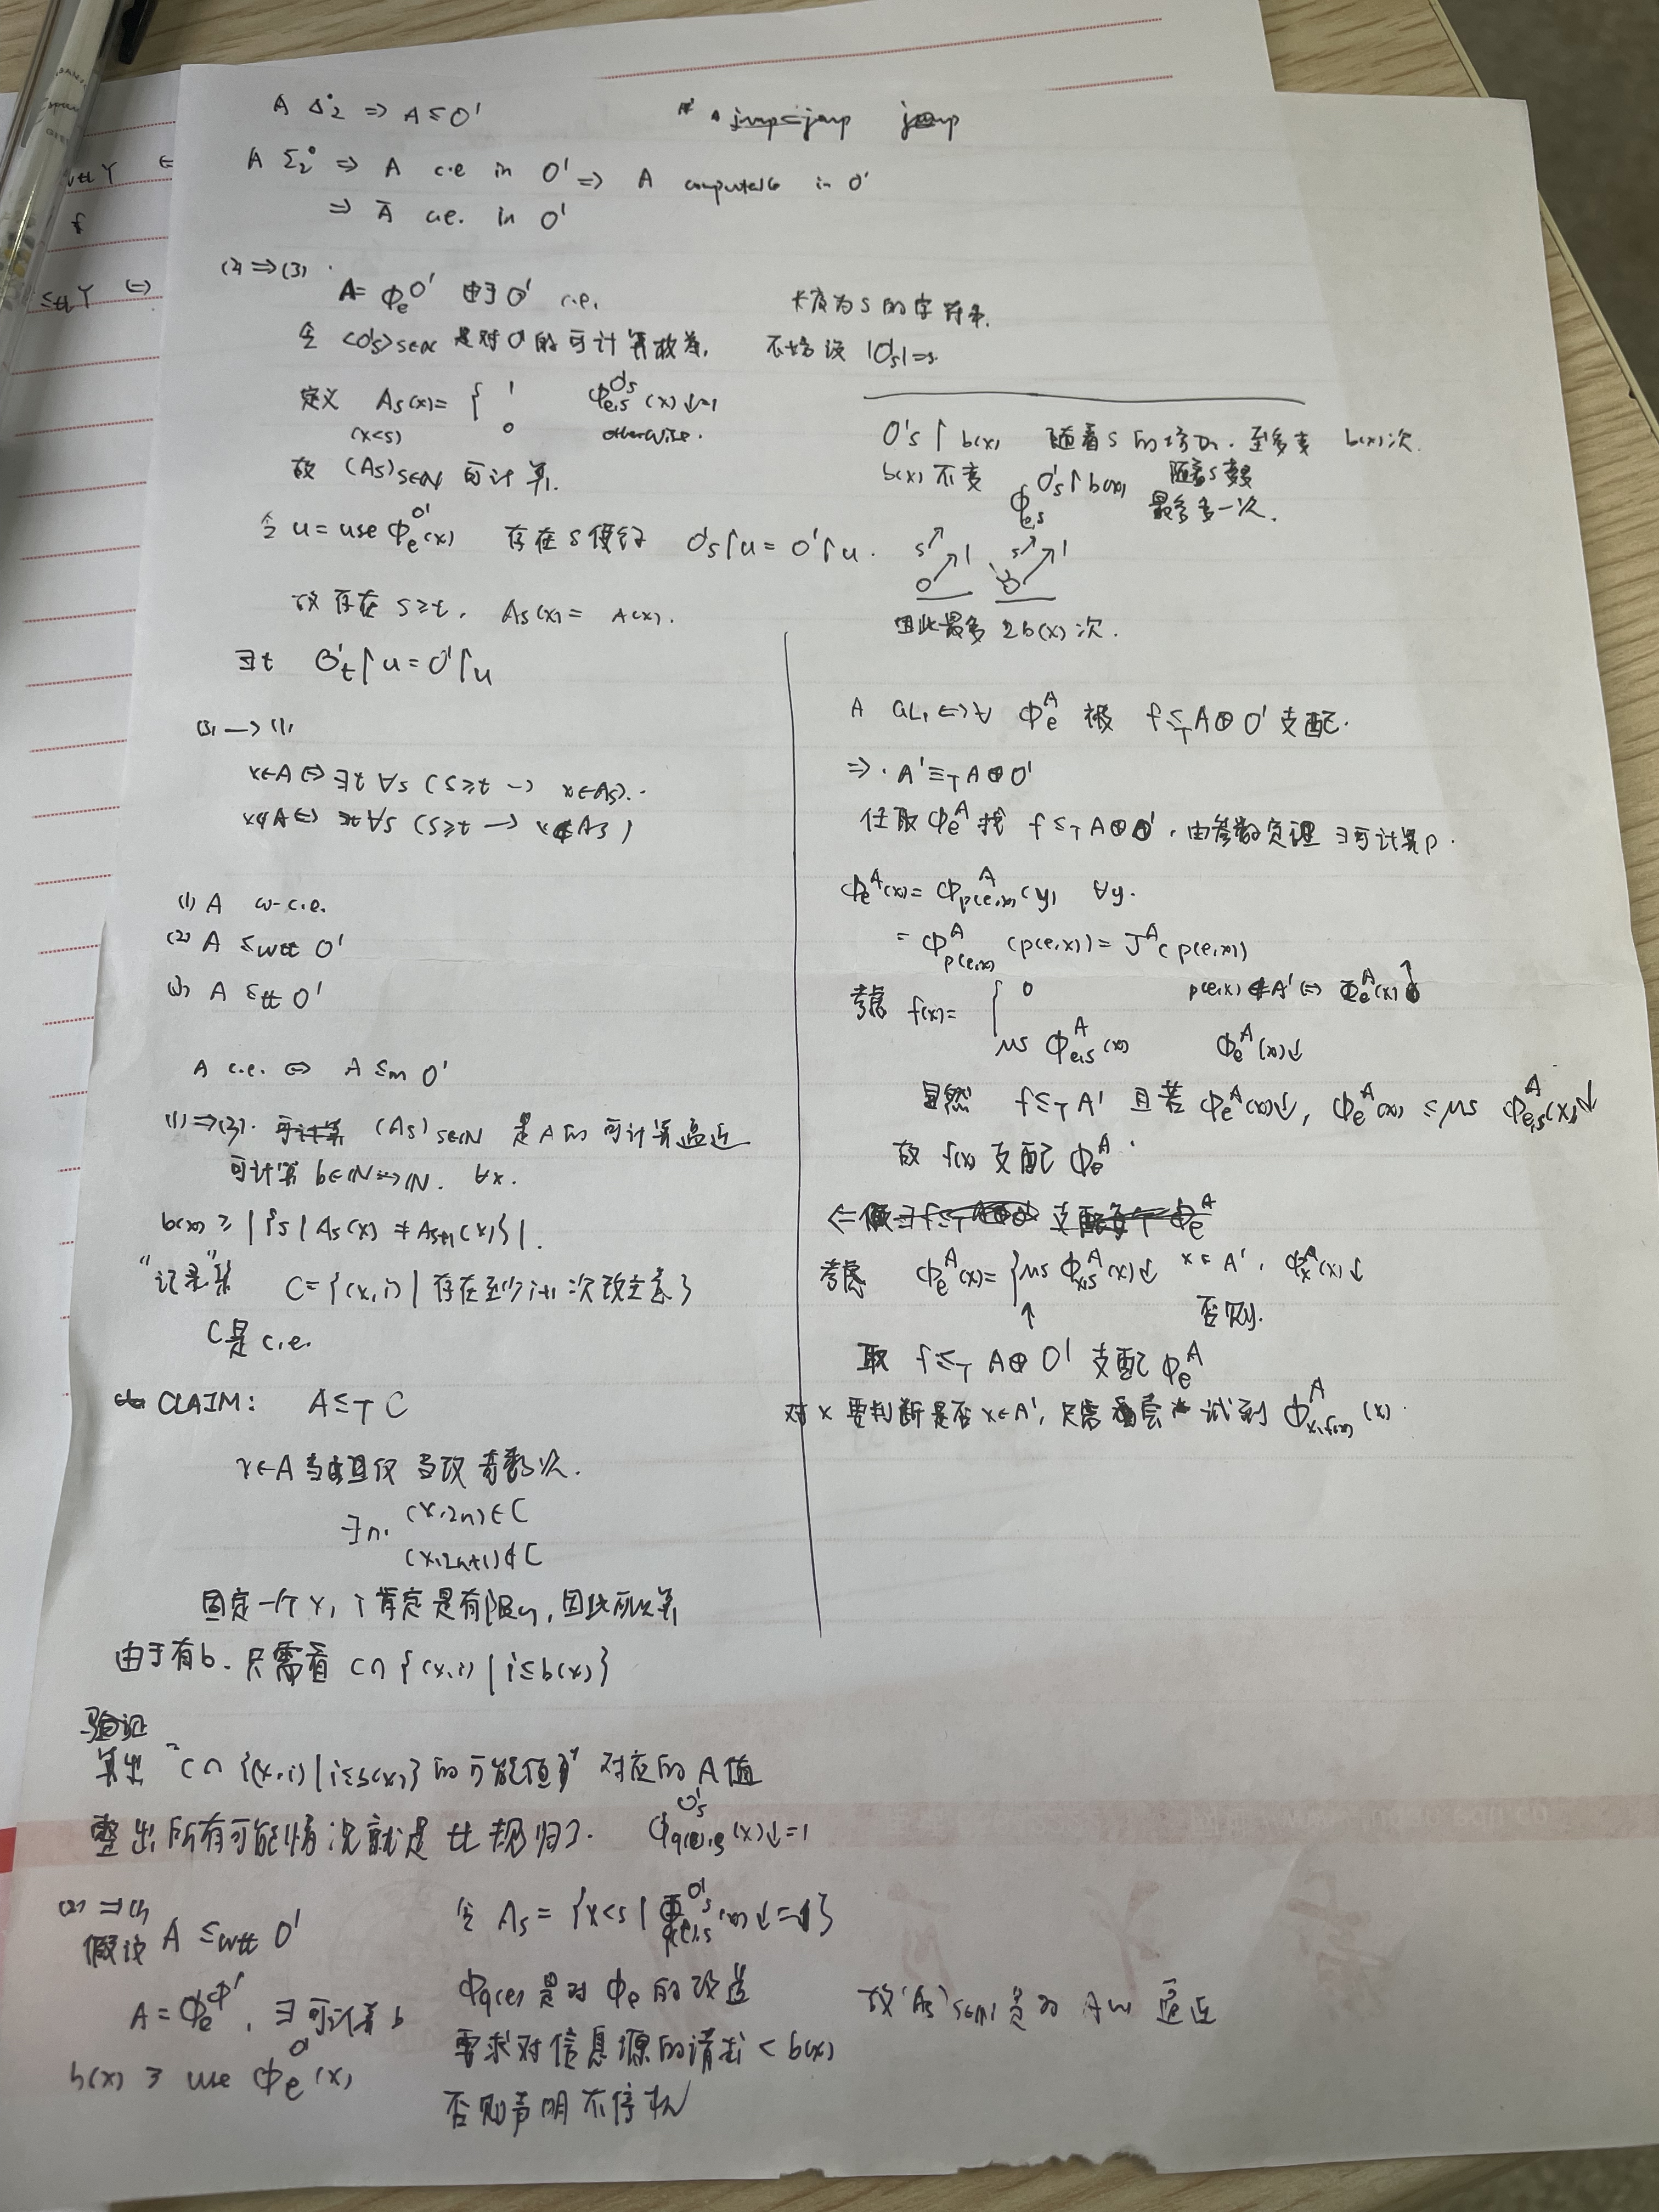
\includegraphics[width=.5\textwidth]{../images/TrivialBigData/1.png}
\label{}
\end{figure}

\begin{equation*}
y=\sigma_\beta(x_1,\dots,x_n)=\sigma(\beta_1x_1+\dots+\beta_nx_n)=\sigma(\beta^Tx)
\end{equation*}
激活函数:\(\sigma(z)=\frac{1}{1+e^{-z}}\)或者\(\sigma(z)=\max\{z,0\}\)或\(\dots\)

\begin{figure}[htbp]
\centering
\includegraphics[width=.6\textwidth]{../images/TrivialBigData/2.png}
\label{}
\end{figure}

神经网络参数\(\beta=(\beta^L,\beta^{L-1},\dots,\beta^1)\)的计算方法:
\begin{gather*}
y=f_\beta(x)=\sigma_{\beta^L}(\sigma_{\beta^{L-1}}(\cdots\sigma_{\beta^1}(x)))\\
C(\beta)=\sum_{i=1}^n(f_\beta(x_i)-y_i)\\
\min_\beta(C(\beta))=\min_\beta\sum_{i=1}^n(f_\beta(x_i)-y_i)^2
\end{gather*}

梯度下降法:
\begin{gather*}
\min_\beta C(\beta)\\
\beta^{k,m+1}=\beta^{k,m}-\lambda\nabla C(\beta^{k,m}),\quad k=1,2,\dots,L
\end{gather*}
记
\begin{equation*}
\beta^{*​,m}=(\beta^{1,m},\beta^{2,m},\dots,\beta^{L,m})
\end{equation*}
\begin{align*}
C(x)&\approx C(x')+\nabla C(x')(x-x')\\
C(\beta^{*​,m+1})&=C(\beta^{*,m}-\lambda\nabla C(\beta^{*,m}))\\
&\approx C(\beta^{*,m})-\lambda\norm{\nabla(\beta^{*,m})}^2\\
&\le C(\beta^{*,m})
\end{align*}
关键在于计算\(C\)关于\(\beta\)的导数,以1维为例,并省略上标\(m\)
\begin{figure}[htbp]
\centering
\includegraphics[width=.8\textwidth]{../images/TrivialBigData/3.png}
\label{}
\end{figure}

\begin{equation*}
x=a^0\to z^1\to a^1\to\dots\to a^{L-1}\to z^L\to z^L
\end{equation*}
其中
\begin{align*}
&z^{i+1}=\beta^{i+1}a^i, i=0,1,\dots,L-1\\
&a^i=\sigma(z^i), i=1,\dots,L\\
&C(\beta)=(a^L-y)^2
\end{align*}
\textbf{需要计算}
\begin{equation*}
\frac{\partial C}{\partial\beta^L},\frac{\partial C}{\partial\beta^{L-1}},\dots,\frac{\partial C}{\partial\beta^1}
\end{equation*}

\begin{align*}
&\frac{\partial C}{\partial a^L}=2(a^L-y)\\
&\frac{\partial C}{\partial\beta^L}=\frac{\partial C}{\partial a^L}\frac{\partial a^L}{\partial z^L}\frac{\partial z^L}{\partial\beta^L}=
2(a^L-y)\cdot \sigma'(z^L)\cdot a^{L-1}
\end{align*}

\begin{align*}
&\frac{\partial C}{\partial a^{L-1}}=\frac{\partial C}{\partial a^L}\frac{\partial a^L}{\partial z^L}\frac{\partial z^L}{\partial a^{L-1}}=
2(a^L-y)\cdot \sigma'(z^L)\cdot \beta^L\\
&\frac{\partial C}{\partial\beta^{L-1}}=\frac{\partial C}{\partial a^{L-1}}\frac{\partial a^{L-1}}{\partial z^{L-1}}\frac{\partial z^{L-1}}{\partial\beta^{L-1}}=
2(a^L-y)\sigma'(z^L)\beta^L\cdot \sigma'(z^{L-1})\cdot a^{L-2}
\end{align*}

因此
\begin{align*}
&\frac{\partial C}{\partial a^i}=\frac{\partial C}{\partial a^{i+1}}\frac{\partial a^{i+1}}{\partial z^{i+1}}\frac{\partial z^{i+1}}{\partial a^i}=
\frac{\partial C}{\partial a^{i+1}}\sigma'(z^{i+1})\beta^{i+1}, \quad i=0,1,\dots,L-1\\
&\frac{\partial C}{\partial\beta^i}=\frac{\partial C}{\partial a^i}\frac{\partial a^i}{\partial z^i}\frac{\partial z^i}{\partial\beta^i}=\frac{\partial C}{\partial a^i}
\sigma'(z^i)a^{i-1},\quad i=1,2,\dots,L
\end{align*}
其中,\(\sigma\)为激活函数,当\(\sigma(z)=\frac{1}{1+e^{-z}}\)时,\(\sigma'(z)=\frac{e^{-z}}{(1+e^{-z})^2}=\sigma(z)(1-\sigma(z))\)

反向传播:
\begin{enumerate}
\item 根据\(\frac{\partial C}{\partial a^L}=2(a^L-y)\)
和\(\frac{\partial C}{\partial a^i}=\frac{\partial C}{\partial a^{i+1}}\sigma'(z^{i+1})\beta^{i+1}\), \(i=0,1,2,\dots,L-1\),反向计算出
\(\frac{\partial C}{\partial a^L},\frac{\partial C}{\partial a^{L-1}},\dots,\frac{\partial C}{\partial a^0}\)
\item 根据\(\frac{\partial C}{\partial\beta^i}=\frac{\partial C}{\partial a^i}\sigma'(z^i)a^{i-1}\), \(i=1,2,\dots,L\),依次计算出
\(\frac{\partial C}{\partial\beta^L},\frac{\partial C}{\partial\beta^{L-1}},\dots,\frac{\partial C}{\partial\beta^1}\)
\item 根据\(\beta^i\leftarrow\beta^i-\lambda\frac{\partial C}{\partial\beta^i}\), \(i=1,2,\dots,L\)对参数进行更新,并重复上述步骤直至收敛。
\end{enumerate}
\end{document}
